\documentclass[11pt]{article}
\usepackage[margin=1in]{geometry}
\usepackage{amsmath,amssymb,amsthm}
\usepackage{graphicx}
\usepackage{booktabs}
\usepackage{caption}
\usepackage[round]{natbib}
\usepackage{setspace}
\usepackage{microtype}
\onehalfspacing

\newtheorem{proposition}{Proposition}
\newtheorem{lemma}{Lemma}
\newtheorem{assumption}{Assumption}
\newtheorem{definition}{Definition}

\title{\textbf{A Credible-Subpopulation Approach to Parallel Trends}}
\author{Parush Arora\\ \small Ashoka University}
\date{\today}

\begin{document}
\maketitle

\begin{abstract}
\noindent Difference-in-differences (DiD) practitioners routinely confront the possibility that
the parallel trends assumption fails for some treated cohorts but not others. The dominant
responses keep the average treatment effect on the treated (ATT) as the target: heterogeneity-robust
estimators point-identify it under parallel trends, while sensitivity methods such as HonestDiD
report a set for it under bounded violations. Both inherit the problem that the ATT may be either
biased or only weakly set-identified when some cohorts violate parallel trends. We propose a
different response: change the estimand. We define a \emph{credible-subpopulation local ATT} (LATT),
the treatment effect for the subpopulation of cohorts whose parallel trends assumption is credible,
and show it is point-identified precisely when the full ATT is not. The procedure is a
reweighting of standard group-time effects toward credible cohorts, combined with honest sensitivity
bounds on the residual violation of the selected set. We are explicit about the method's scope: its
advantage over the ATT grows with how informative pre-trends are about post-treatment violations and
vanishes when they are uninformative, where only economic context can carry the identifying
assumption. A reduced-form and a panel simulation study confirm that the LATT recovers a clean effect
where the ATT estimator is biased, that the sensitivity bounds restore honest coverage where point
estimates collapse, and that a relative-magnitudes restriction is self-undermining under uninformative
pre-trends while a smoothness restriction is not.
\end{abstract}

\section{Introduction}

Difference-in-differences is among the most widely used research designs in empirical economics, and
a large recent literature has clarified both its assumptions and its failure modes
\citep{roth2023trending}. The design's credibility rests on the parallel trends assumption: absent
treatment, the average outcomes of treated and comparison units would have evolved in parallel. In
practice researchers are rarely certain this holds, and it has become standard to assess it by
testing for pre-treatment differences in trends. As \citet{roth2023trending} synthesize, this
pre-testing practice is fragile: pre-trends tests are often underpowered against economically
meaningful violations \citep{kahnlang2020, roth2022pretrends}, conditioning on passing them induces a
pre-test selection bias \citep{roth2022pretrends}, and even a clean pre-period does not guarantee a
clean post-period \citep{kahnlang2020}.

Two strands of methodology respond to this concern, and both retain the ATT as the estimand. The
first develops heterogeneity-robust estimators for staggered adoption
\citep{callaway2021, sun2021, borusyak2024, dechaisemartin2020, goodmanbacon2021}, which point-identify
interpretable aggregations of group-time effects under a suitable parallel trends assumption but remain
biased if that assumption fails. The second, exemplified by \citet{rambachan2023}, abandons exact
parallel trends and instead bounds how different post-treatment violations can be from the observed
pre-trends, reporting a uniformly valid confidence \emph{set} for the ATT. This is a substantial
advance, but it inherits a structural limitation: when parallel trends fails for some cohorts, the
ATT---an average over \emph{all} treated cohorts, including the offending ones---is precisely the
object that is hard to recover. The heterogeneity-robust point estimate is then biased, and the
HonestDiD set can be wide and uninformative, because it must accommodate the worst offenders.

This paper takes a different route, familiar from other corners of causal inference: when the
population target is not credibly identified, retreat to a subpopulation where it is. This is the
logic of the local average treatment effect \citep{imbens1994}, of the optimal-subpopulation average
treatment effect under limited overlap \citep{crump2009}, and of overlap weighting \citep{li2018}. In
each case one trades the original estimand for a credibly-identified effect on a selected
subpopulation, and defends the trade by characterizing whom the subpopulation comprises. We develop
the staggered-DiD instance of this principle. We define the credible-subpopulation LATT---the
weighted average of group-time effects restricted to cohorts whose parallel trends assumption is
credible---and show that it is point-identified even when the full ATT is not, because the violations
of the excluded cohorts do not enter it. Estimation is a transparent reweighting of the
\citet{callaway2021} group-time effects; the credibility of a cohort is assessed from its pre-trends,
so that the reweighting is a data-dependent selection, and we treat inference on the selected set with
the sensitivity machinery of \citet{rambachan2023}.

Our contribution is therefore primarily one of framing and estimand choice rather than of new
estimation or inference technology, and we are deliberate about this. The method occupies a distinct
point on a credibility--precision--scope frontier: relative to a heterogeneity-robust point estimate
of the ATT it gives up scope (it targets a subpopulation) to buy back credibility; relative to a
HonestDiD set for the ATT it gives up nothing in honesty but recovers a sharper, point-identified
answer to a narrower question. We are equally explicit about the method's limits. Its advantage is
governed by how informative pre-trends are about post-treatment violations; when they are
uninformative, selecting on them buys nothing, and the identifying assumption must be carried by
economic context rather than by the data. We show, moreover, that the natural relative-magnitudes
sensitivity restriction is \emph{self-undermining} in exactly this regime---it anchors its bounds to
the observed pre-trends and so reports false precision when those pre-trends are flat---whereas a
smoothness restriction, which keys off structure rather than magnitude, is not.

The remainder of the paper is organized as follows. Section~\ref{sec:setup} fixes the staggered-DiD
setup and the decomposition of event-study coefficients into a causal and a differential-trend
component. Section~\ref{sec:approach} defines the credible-subpopulation LATT, states its
identification and the properties of its estimator, and gives our recommended sensitivity-based
inference together with an honest account of what is provable and what is not.
Section~\ref{sec:sim} reports the simulation study. Section~\ref{sec:conc} concludes.

\section{Setup}\label{sec:setup}

We adopt the staggered adoption framework of \citet{callaway2021}. There are periods
$t=1,\dots,T$ and units $i$ indexed by their first treatment date $G_i \in \{2,\dots,T\}\cup\{\infty\}$,
where $G_i=\infty$ denotes never-treated. Let $Y_{it}(g)$ denote the potential outcome in period $t$
if unit $i$ is first treated in period $g$, and $Y_{it}(\infty)$ the never-treated potential outcome.
The building-block causal parameter is the group-time average treatment effect on the treated,
\begin{equation}
\mathrm{ATT}(g,t) = \mathbb{E}\!\left[\,Y_{it}(g)-Y_{it}(\infty)\mid G_i=g\,\right].
\end{equation}
Summary parameters are weighted aggregations $\theta = \sum_{g}\sum_t w(g,t)\,\mathrm{ATT}(g,t)$ with
researcher-chosen weights, of which the overall ATT and the event-study path are special cases.

It is convenient to work with the event-study representation and the decomposition of
\citet{rambachan2023}. Let $\hat\beta=(\hat\beta_{\mathrm{pre}}',\hat\beta_{\mathrm{post}}')'$ be an
asymptotically normal vector of event-study coefficients estimated by any of the heterogeneity-robust
procedures above, with $\sqrt{n}(\hat\beta-\beta)\to\mathcal{N}(0,\Sigma)$. The estimand decomposes as
\begin{equation}
\beta = \tau + \delta, \qquad \tau_{\mathrm{pre}}=0,
\label{eq:decomp}
\end{equation}
where $\tau$ collects the causal effects (zero before treatment, by no anticipation) and $\delta$ is
the differential trend between treated and comparison groups that would have occurred absent
treatment. Parallel trends is the restriction $\delta_{\mathrm{post}}=0$, under which
$\beta_{\mathrm{post}}=\tau_{\mathrm{post}}$; a pre-trends test is a test of $\delta_{\mathrm{pre}}=0$.

We will require the analogous objects at the cohort level. Write $\delta_g$ for the differential
trend of cohort $g$ and say that parallel trends \emph{holds for $g$} if $\delta_{g,\mathrm{post}}=0$.
A key feature of applications is that this may hold for some cohorts and fail for others: a policy
adopted by cohort $g$ may be as good as randomly timed while another cohort's adoption coincides with
a confounding shock.

Finally, we distinguish two regimes for how cohorts are judged credible, because they carry different
inferential guarantees. Under \emph{ex-ante} (or independent) selection, credibility is decided from
pre-determined covariates, institutional knowledge, or an independent data split, so that the selected
set is statistically independent of the estimation errors in $\hat\beta$. Under \emph{data-driven}
selection, credibility is assessed from the realized pre-trends $\hat\beta_{\mathrm{pre}}$, so that the
selected set depends on the estimation sample. The distinction is immaterial for the estimand and its
identification, but central for inference, and we treat it explicitly in
Section~\ref{sec:approach}.

\section{The credible-subpopulation LATT: approach and recommendations}\label{sec:approach}

\subsection{Estimand and identification}

Let $S$ denote a set of cohorts judged to have credible parallel trends, produced by a selection rule
$R$ that we specify below. We define the target as the treatment effect for that subpopulation.

\begin{definition}[Credible-subpopulation LATT]
For cohort weights $w_g>0$ (e.g.\ proportional to cohort size), the credible-subpopulation local ATT is
\begin{equation}
\theta_S \;=\; \frac{\sum_{g\in S} w_g\,\mathrm{ATT}(g,\cdot)}{\sum_{g\in S} w_g},
\end{equation}
where $\mathrm{ATT}(g,\cdot)$ is any within-cohort aggregation of interest (a fixed event-time, or an
average over post-treatment periods).
\end{definition}

The value of the target is that it is identified under a weaker condition than the ATT.

\begin{proposition}[Identification]\label{prop:id}
If parallel trends holds for every $g\in S$, i.e.\ $\delta_{g,\mathrm{post}}=0$ for all $g\in S$, then
$\theta_S$ is point-identified by the reweighted group-time effects,
$\theta_S = \big(\sum_{g\in S} w_g\,\beta_{g,\mathrm{post}}\big)/\sum_{g\in S} w_g$, and this holds
irrespective of whether $\delta_{g,\mathrm{post}}\neq 0$ for cohorts $g\notin S$.
\end{proposition}

\begin{proof}
For $g\in S$, $\beta_{g,\mathrm{post}} = \tau_{g,\mathrm{post}}+\delta_{g,\mathrm{post}}
= \tau_{g,\mathrm{post}}$ by the hypothesis and \eqref{eq:decomp}. The reweighted sum over $S$ therefore
equals the corresponding weighted average of causal effects, which is $\theta_S$ by definition. Cohorts
outside $S$ receive zero weight, so their differential trends do not enter.
\end{proof}

Proposition~\ref{prop:id} is elementary, but it is the paper's central point: by \emph{changing the
target} to the credible subpopulation, one converts a partially-identified problem (the ATT, when some
cohorts violate parallel trends) into a point-identified one, at the cost of answering a narrower
question. This is exactly the trade made by \citet{imbens1994}, \citet{crump2009}, and \citet{li2018}
in other settings, and it carries the same interpretive obligation: one must characterize the
subpopulation $S$ that the estimand describes.

\subsection{Estimation}

The estimator $\hat\theta_S$ replaces population objects by their \citet{callaway2021} sample
analogues and reweights over the selected cohorts. Its large-sample behavior is standard under ex-ante
selection.

\begin{proposition}[Consistency and efficiency]\label{prop:cons}
Under ex-ante selection and the regularity conditions of \citet{callaway2021}, $\hat\theta_S$ is
consistent for $\theta_S$. If parallel trends holds for all cohorts, $\hat\theta_S$ is consistent for
the ATT, with an efficiency loss relative to estimators that use all cohorts.
\end{proposition}

Under data-driven selection the selected set is random and correlated with the estimation errors,
which introduces a finite-sample pre-test bias of the kind analyzed by \citet{roth2022pretrends}.

\begin{proposition}[Pre-test bias]\label{prop:pretest}
Under data-driven selection, $\hat\theta_S$ carries a finite-sample bias that vanishes as the
per-cohort information grows and the selection rule becomes consistent for the credible set.
\end{proposition}

We emphasize, consistent with Proposition~\ref{prop:pretest} and with our simulations below, that the
honest claim is consistency, not finite-sample unbiasedness: the data-driven estimator is close to,
but not exactly on, the target in small samples, and the gap closes with sample size.

\subsection{Honest inference on the selected set}

Selecting credible cohorts does not by itself deliver parallel trends: a cohort with flat pre-trends
may still have a nonzero post-treatment differential trend, and the selection removes gross offenders
but not subtle residual violations. We therefore recommend accompanying the point estimate with the
sensitivity analysis of \citet{rambachan2023}, applied to the \emph{selected-cohort aggregate}
event study. Concretely, one imposes a restriction $\delta_{S,\mathrm{post}}\in\Delta$ on the residual
differential trend of the selected set and reports the implied confidence set for $\theta_S$. Among the
restrictions of \citet{rambachan2023}, the smoothness class
$\Delta^{SD}(M)=\{\delta:\lvert\delta_{t+1}-2\delta_t+\delta_{t-1}\rvert\le M\ \forall t\}$ admits the
fixed-length confidence intervals (FLCIs) of \citet{armstrong2018}, which are near-optimal for convex
centrosymmetric restrictions and which we adopt.

The validity of this step depends on the selection regime. Under ex-ante selection the selected set is
independent of $\hat\beta$, so the uniform validity results of \citet{rambachan2023} apply verbatim to
the selected-cohort event study, and no new inference theory is required. Under data-driven selection
the situation is more delicate: the selection is a function of $\hat\beta_{\mathrm{pre}}$, and a
classical impossibility result of \citet{leeb2005} precludes uniformly valid inference from the naive
post-selection estimator without conditioning, sample-splitting, or randomization. Our simulations
(Section~\ref{sec:sim}) find that in practice the data-driven procedure exhibits no systematic
coverage distortion---full-data and split implementations cover almost identically---so that the naive
procedure is typically valid; but this is a pointwise, not a worst-case uniform, statement, and we are
explicit about the distinction. A researcher who requires a worst-case guarantee can obtain it cheaply
by selecting on pre-determined information, by splitting the sample, or by randomized (data-carving)
selection in the sense of \citet{fithian2014}, all of which restore the independence that
Proposition~\ref{prop:id}'s inferential counterpart needs.

A further subtlety arises because the selected set is random. The FLCI at bound $M$ is valid for a
given selected set only if that set's residual differential trend lies in $\Delta^{SD}(M)$; since the
set is random, its residual curvature is a random variable, and unconditional coverage requires $M$ to
dominate that variable with high probability.

\begin{lemma}[Calibration to the random selected set]\label{lem:calib}
Under data-driven selection, choosing $M$ equal to the \emph{mean} residual curvature of the selected
aggregate undercovers; unconditional coverage requires $M$ to exceed the mean and to approach an upper
quantile of the residual-curvature distribution, with the FLCI's sampling slack providing a partial
buffer.
\end{lemma}

Lemma~\ref{lem:calib} is confirmed sharply in Section~\ref{sec:sim} and is a practical warning: the
sensitivity bound must be set conservatively relative to the \emph{typical} selected set, not merely
to satisfy it on average.

Finally, we caution against one otherwise-natural choice of $\Delta$. The relative-magnitudes
restriction $\Delta^{RM}(\bar M)$ of \citet{rambachan2023}, following \citet{manski2018}, bounds
post-treatment violations by $\bar M$ times the observed maximal pre-treatment violation. Because it
anchors its bound to the observed pre-trends, it is self-undermining precisely in the regime where our
method's value is in question.

\begin{proposition}[Relative magnitudes is self-undermining]\label{prop:rm}
The identified-set half-width under $\Delta^{RM}(\bar M)$ is proportional to the observed pre-trend
magnitude. When pre-trends are uninformative about post-treatment violations, the observed pre-trends
are small while the true violation need not be, so $\Delta^{RM}(\bar M)$ produces intervals whose width
tends to zero even as the bias does not, yielding undercoverage. A structural restriction such as
$\Delta^{SD}(M)$ does not share this defect, since its bound keys off smoothness rather than pre-trend
magnitude.
\end{proposition}

\subsection{Scope: when to prefer the LATT}

The method's advantage over the ATT is not uniform; it is governed by how informative pre-trends are
about post-treatment violations. When they are informative, selecting on them isolates credible
cohorts and the LATT recovers a clean effect while the ATT estimator remains biased. When they are
uninformative, selection is uninformative about the post-period, the residual violation of the selected
set is as large as for any set, and the method offers no advantage over the ATT---there is no free
lunch, and the identifying assumption must be defended from economic context. We regard a formal
decision-theoretic characterization of the region in which the point-identified LATT dominates the
set-valued ATT, in the sense of \citet{armstrong2018}, as the principal open theoretical question; the
simulations below map its empirical shadow.

\section{Simulation study}\label{sec:sim}

We study the method in a reduced-form normal model, in which event-study coefficients are drawn
directly from their asymptotic distribution, and in a full panel micro-simulation, in which
individual data are generated and the coefficients and their covariance are estimated. The reduced-form
model isolates the inferential mechanics, where the underlying theory is exact; the panel model
confirms that the conclusions survive realistic estimation.

\subsection{The estimand: recovering a clean effect where the ATT is biased}

We first illustrate Proposition~\ref{prop:id}. Twelve cohorts share a common true effect of one; a
subset violate parallel trends in the post-period, biasing any estimator of the ATT. A
heterogeneity-robust estimator of the ATT and the reweighted LATT are compared to the truth.
Table~\ref{tab:tier1} reports the result. The ATT estimator is biased by $+0.27$, entirely on account
of the offending cohorts, while the LATT recovers the credible-subpopulation effect. The right panel
sweeps the sampling precision: the LATT's bias vanishes as precision grows---the pre-test bias of
Proposition~\ref{prop:pretest}---whereas the ATT estimator's bias is frozen, because it is a
wrong-target problem, not a noise problem.

\begin{table}[t]
\centering
\caption{The estimand demonstration (reduced-form model). True effect $=1$ for all cohorts.}
\label{tab:tier1}
\begin{tabular}{lcc}
\toprule
& ATT estimator & LATT (ours) \\
\midrule
Point estimate & $1.267$ & $1.013$ \\
Bias vs.\ truth & $+0.267$ & $+0.013$ \\
\midrule
\multicolumn{3}{l}{\emph{Bias as sampling noise $s$ falls:}}\\
$s=0.40$ & $+0.269$ & $+0.048$ \\
$s=0.20$ & $+0.267$ & $+0.005$ \\
$s=0.12$ & $+0.267$ & $+0.000$ \\
$s=0.03$ & $+0.267$ & $-0.000$ \\
\bottomrule
\end{tabular}
\end{table}

\subsection{The scope condition}

Figure~\ref{fig:scope} traces the method across the axis that governs it: the informativeness of
pre-trends about post-treatment violations. The bias of the ATT estimator is flat---it never consults
pre-trends---while the LATT's advantage is the vertical gap between the two, zero when pre-trends are
uninformative and maximal when they are informative. The lower-left panel shows that the causal
coverage of a point-based interval collapses at low informativeness; crucially, this collapse is
driven by the residual violation of the surviving cohorts (an identification gap), not by selection
distortion, since sample-splitting---which removes selection distortion by construction---collapses
identically. This motivates the sensitivity bounds of the next subsection, and confirms that when
pre-trends are uninformative the method correctly reports no advantage.

\begin{figure}[t]
\centering
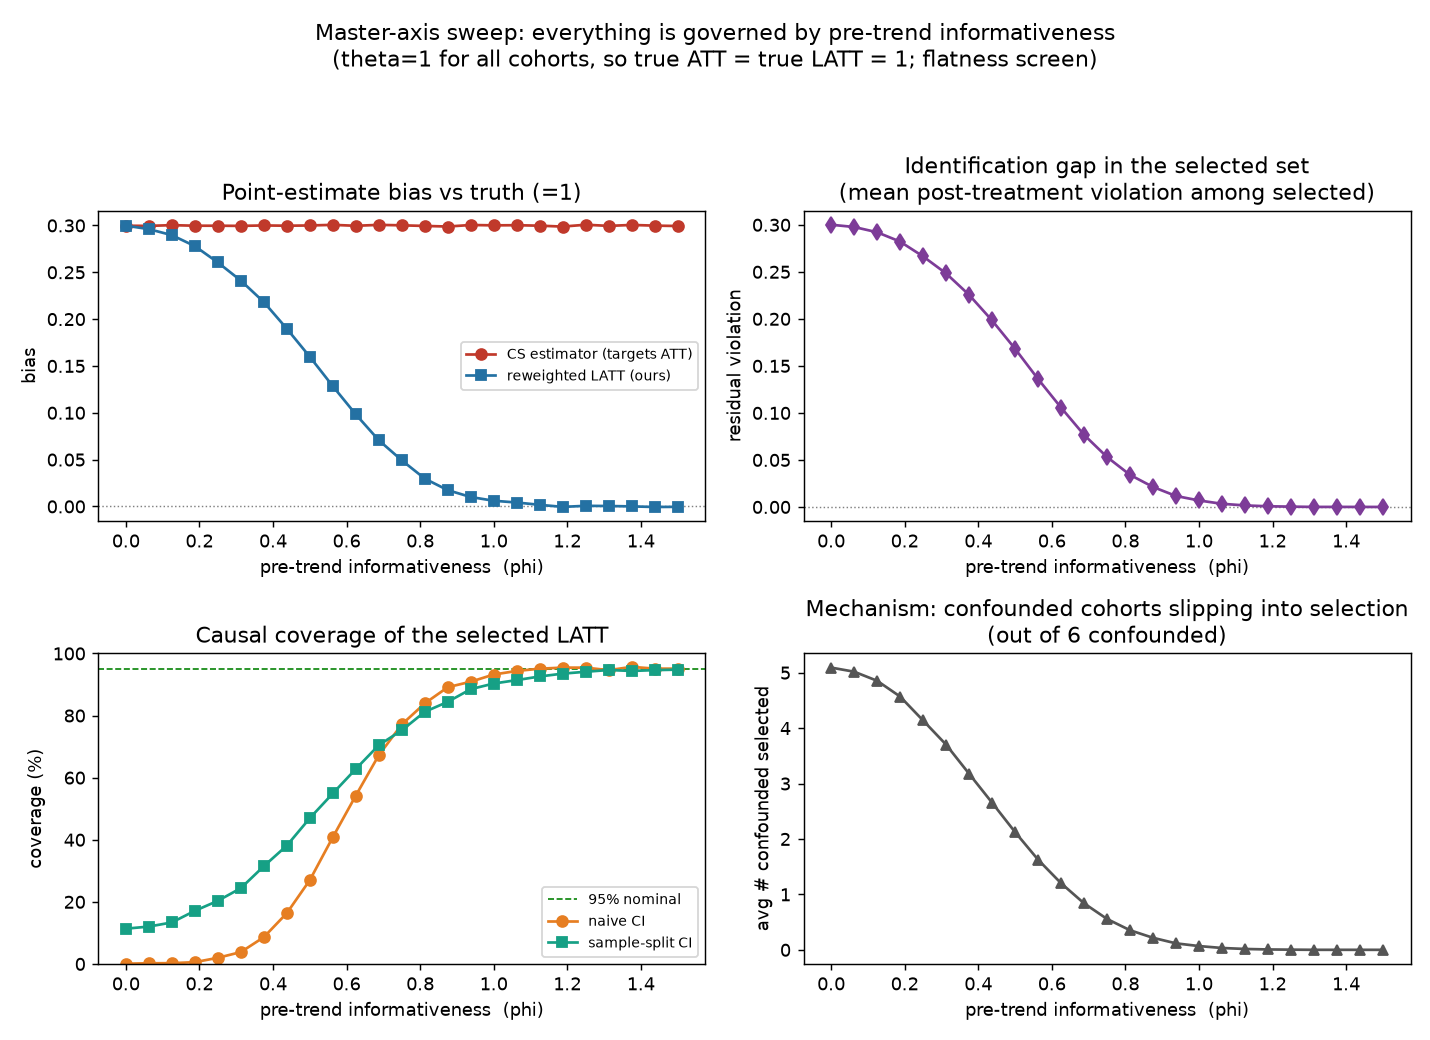
\includegraphics[width=\textwidth]{master_axis.png}
\caption{Scope condition. Everything is governed by pre-trend informativeness. The ATT estimator's
bias is constant; the LATT's advantage is the gap between the lines. Causal-coverage collapse at low
informativeness is an identification gap (surviving cohorts still violate parallel trends), not
selection distortion---sample-splitting collapses identically.}
\label{fig:scope}
\end{figure}

\subsection{Honest inference restores coverage}

We validate the smoothness-class FLCI applied to the selected aggregate. Table~\ref{tab:flci} confirms
the exact honest behavior: the FLCI covers when and only when the assumed bound $M$ dominates the true
residual curvature $C$, while both a naive point interval and a linear-extrapolation point interval
collapse to zero coverage the instant any curvature is present. Figure~\ref{fig:layer2} shows the same
result across a continuum of curvature: the point estimates collapse as the confound curves, the FLCIs
remain honest exactly up to their assumed $M$, the price of honesty is interval width set by $M$, and
the sensitivity curve delivers an interpretable breakdown value. Because $\Delta^{SD}(M)$ keys off
smoothness rather than pre-trend magnitude, this honesty does not degrade with informativeness---in
contrast to the relative-magnitudes restriction of Proposition~\ref{prop:rm}.

\begin{table}[t]
\centering
\caption{FLCI coverage of the causal target (reduced-form model): valid iff $M\ge C$.}
\label{tab:flci}
\begin{tabular}{cccc}
\toprule
True curvature $C$ & Assumed $M$ & FLCI coverage & Point-estimate coverage \\
\midrule
$0.5$ & $0.5\ (=C)$ & $94.7\%$ & $0.0\%$ \\
$0.5$ & $1.0\ (>C)$ & $100\%$ & $0.0\%$ \\
$1.0$ & $0.5\ (<C)$ & $0.0\%$ & $0.0\%$ \\
$1.0$ & $1.0\ (=C)$ & $95.2\%$ & $0.0\%$ \\
\bottomrule
\end{tabular}
\end{table}

\begin{figure}[t]
\centering
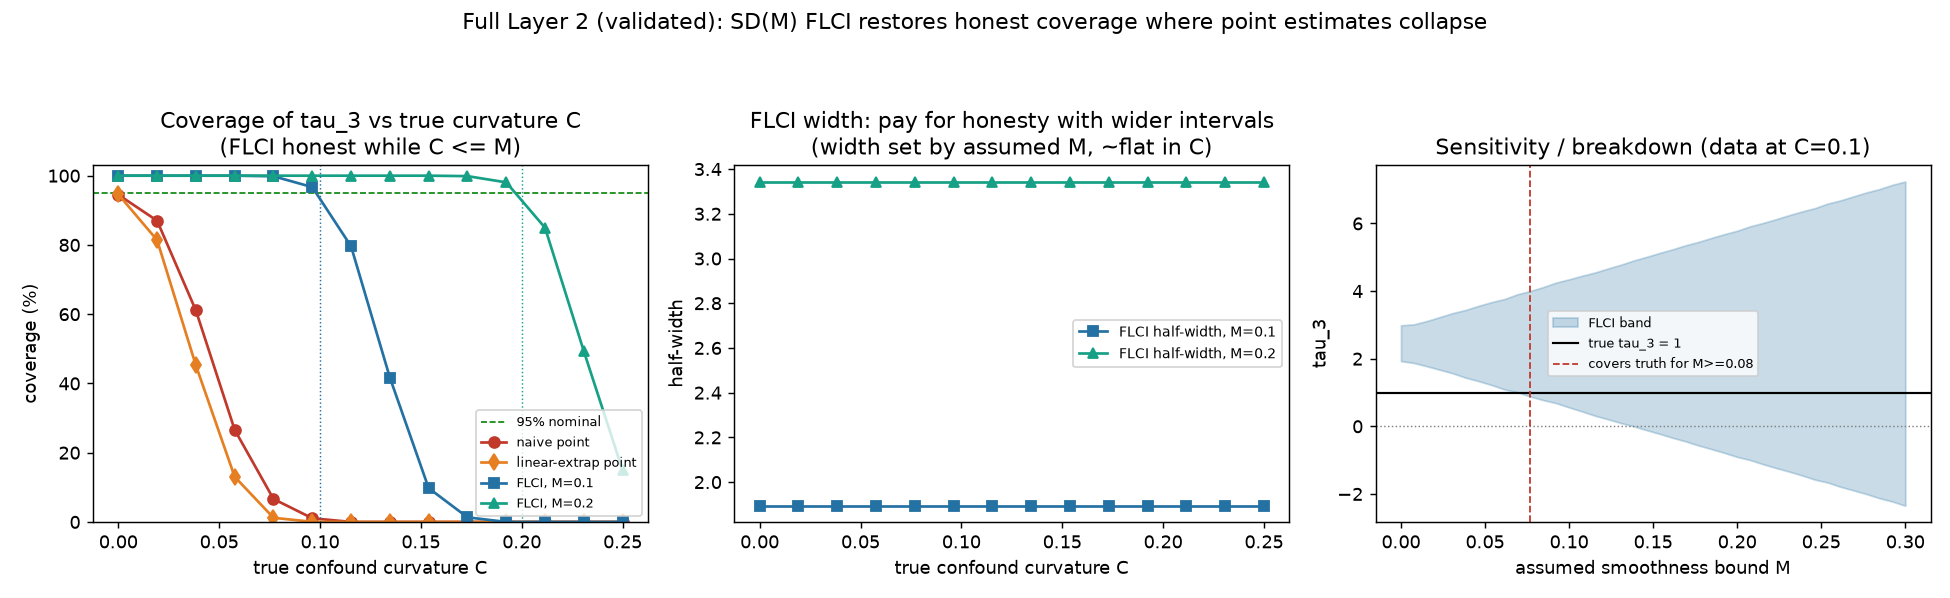
\includegraphics[width=\textwidth]{layer2_full.png}
\caption{Sensitivity bounds restore honest coverage. Point estimates collapse as the confound curves;
the FLCI is honest exactly while $M\ge C$; interval width is the price of honesty, set by $M$; the
right panel is the sensitivity/breakdown curve.}
\label{fig:layer2}
\end{figure}

\subsection{Selection does not distort the bounds, but calibration must respect randomness}

Two questions remain for the data-driven regime: does selection distort the FLCI, and how should $M$ be
chosen given that the selected set is random. Figure~\ref{fig:calib} answers both. Full-data selection
and sample-splitting cross nominal coverage at the same bound, so selection introduces no systematic
distortion of the FLCI---consistent with the pointwise reading of \citet{leeb2005} in favorable
regimes, and confirming that splitting is not needed on this account. At the same time, a bound $M$
set to the \emph{mean} residual curvature of the selected set ($0.031$) undercovers, reaching only
about $88\%$; nominal coverage is attained at $M\approx0.039$, above the mean though below the strict
maximum ($0.050$), as Lemma~\ref{lem:calib} anticipates. The practical recommendation is to calibrate
$M$ to the typical selected set, not to its average.

\begin{figure}[t]
\centering

\includegraphics[width=\textwidth]{m_sweep.png}
\caption{Calibrating the sensitivity bound to the random selected set. Full-data and split coverage
cross nominal at the same $M$ (no selection distortion); a mean-calibrated $M$ undercovers, with
nominal coverage reached above the mean residual curvature.}
\label{fig:calib}
\end{figure}

\subsection{Panel confirmation}

The reduced-form conclusions survive the full panel micro-simulation, in which individual outcomes are
generated for a staggered design, cohort-level pre- and post-treatment coefficients are estimated
against a common never-treated control, and the covariance is estimated from the data. The estimand
demonstration is unchanged---the ATT estimator's bias is flat near $+0.30$ while the LATT's bias falls
toward zero with precision---and the estimated covariance is well calibrated where selection is
deterministic. The residual gap at intermediate informativeness reflects the selection-induced
component of variance that a conditional standard error omits, an independent confirmation of the
inferential issues discussed above.

\section{Conclusion}\label{sec:conc}

We have argued that when parallel trends fails for some treated cohorts, a productive response is to
change the estimand rather than to defend or bound the ATT. The credible-subpopulation LATT is
point-identified precisely when the ATT is not, is estimated by a transparent reweighting of standard
group-time effects, and can be accompanied by honest sensitivity bounds on the residual violation of
the selected set. The approach is a specific instance of a general principle---retreat to a
credibly-identified subpopulation---already established in the analysis of instrumental variables and
of limited overlap.

We have been explicit about the method's advantages and its weaknesses. Its advantage over the ATT is
that it delivers a sharp, credibly-identified answer where the ATT estimator is biased and the
ATT sensitivity set is wide; its transparency about which comparisons identify the effect is inherited
from \citet{callaway2021}. Its weaknesses are equally concrete. The estimand is a subpopulation effect
and must be interpreted as such, with the composition of the credible set described rather than assumed
away. Its advantage is contingent on pre-trends being informative about post-treatment violations, and
when they are not, only economic context can carry the identifying assumption. Under data-driven
selection the estimator carries a vanishing pre-test bias, and worst-case uniform inference is
precluded without ex-ante selection, sample-splitting, or randomization---though we find no systematic
distortion in practice. The sensitivity bound must be calibrated to the typical selected set, and the
relative-magnitudes restriction should be avoided in favor of a structural one, since the former is
self-undermining under uninformative pre-trends.

The principal open question is theoretical: a decision-theoretic characterization of the region in
which the point-identified LATT dominates the set-valued ATT would convert the empirical scope
condition documented here into a formal recommendation, and would sharpen the choice between the two
responses to imperfect parallel trends. We regard the framing developed here---estimand choice as the
lever, with credibility purchased by narrowing the target---as the paper's contribution, and the
accompanying honesty about scope as inseparable from it.

\begin{thebibliography}{99}
\small
\bibitem[Armstrong and Koles\'ar(2018)]{armstrong2018} Armstrong, T.~B. and M.~Koles\'ar (2018).
Optimal inference in a class of regression models. \emph{Econometrica} 86(2), 655--683.

\bibitem[Borusyak et~al.(2024)]{borusyak2024} Borusyak, K., X.~Jaravel, and J.~Spiess (2024).
Revisiting event-study designs: robust and efficient estimation. \emph{Review of Economic Studies},
forthcoming.

\bibitem[Callaway and Sant'Anna(2021)]{callaway2021} Callaway, B. and P.~H.~C. Sant'Anna (2021).
Difference-in-differences with multiple time periods. \emph{Journal of Econometrics} 225(2), 200--230.

\bibitem[Crump et~al.(2009)]{crump2009} Crump, R.~K., V.~J. Hotz, G.~W. Imbens, and O.~A. Mitnik
(2009). Dealing with limited overlap in estimation of average treatment effects. \emph{Biometrika}
96(1), 187--199.

\bibitem[de Chaisemartin and D'Haultf\oe uille(2020)]{dechaisemartin2020} de Chaisemartin, C. and
X.~D'Haultf\oe uille (2020). Two-way fixed effects estimators with heterogeneous treatment effects.
\emph{American Economic Review} 110(9), 2964--2996.

\bibitem[Fithian et~al.(2014)]{fithian2014} Fithian, W., D.~Sun, and J.~Taylor (2014). Optimal
inference after model selection. \emph{arXiv:1410.2597}.

\bibitem[Goodman-Bacon(2021)]{goodmanbacon2021} Goodman-Bacon, A. (2021). Difference-in-differences
with variation in treatment timing. \emph{Journal of Econometrics} 225(2), 254--277.

\bibitem[Imbens and Angrist(1994)]{imbens1994} Imbens, G.~W. and J.~D. Angrist (1994). Identification
and estimation of local average treatment effects. \emph{Econometrica} 62(2), 467--475.

\bibitem[Kahn-Lang and Lang(2020)]{kahnlang2020} Kahn-Lang, A. and K.~Lang (2020). The promise and
pitfalls of differences-in-differences. \emph{Journal of Business \& Economic Statistics} 38(3),
613--620.

\bibitem[Leeb and P\"otscher(2005)]{leeb2005} Leeb, H. and B.~M. P\"otscher (2005). Model selection and
inference: facts and fiction. \emph{Econometric Theory} 21(1), 21--59.

\bibitem[Li et~al.(2018)]{li2018} Li, F., K.~L. Morgan, and A.~M. Zaslavsky (2018). Balancing
covariates via propensity score weighting. \emph{Journal of the American Statistical Association}
113(521), 390--400.

\bibitem[Manski and Pepper(2018)]{manski2018} Manski, C.~F. and J.~V. Pepper (2018). How do right-to-carry
laws affect crime rates? Coping with ambiguity using bounded-variation assumptions. \emph{Review of
Economics and Statistics} 100(2), 232--244.

\bibitem[Rambachan and Roth(2023)]{rambachan2023} Rambachan, A. and J.~Roth (2023). A more credible
approach to parallel trends. \emph{Review of Economic Studies} 90(5), 2555--2591.

\bibitem[Roth(2022)]{roth2022pretrends} Roth, J. (2022). Pretest with caution: event-study estimates
after testing for parallel trends. \emph{American Economic Review: Insights} 4(3), 305--322.

\bibitem[Roth et~al.(2023)]{roth2023trending} Roth, J., P.~H.~C. Sant'Anna, A.~Bilinski, and J.~Poe
(2023). What's trending in difference-in-differences? A synthesis of the recent econometrics
literature. \emph{Journal of Econometrics} 235(2), 2218--2244.

\bibitem[Sun and Abraham(2021)]{sun2021} Sun, L. and S.~Abraham (2021). Estimating dynamic treatment
effects in event studies with heterogeneous treatment effects. \emph{Journal of Econometrics} 225(2),
175--199.
\end{thebibliography}

\end{document}
